%! Author = angel
%! Date = 1/28/25

% Preamble
\documentclass[11pt]{article}

% Packages
\usepackage{amsmath,amssymb,amsthm}
\usepackage[letterpaper,margin=0.75in]{geometry}
\usepackage{pgfplots}
\usepackage{tikz}
\usepackage{xcolor}
\usepackage{fancyhdr}
\pgfplotsset{compat=1.18}
% Document



\begin{document}
    \noindent \textbf{Chapter 17 - Waves II}
    \\ \noindent \newline Sound waves fall are considered longitudinal waves modeled by the equation:
    \begin{equation}
        s(x,t) = s_m\cos(kx - \omega t + \phi) \tag{sound equation}
    \end{equation}


    \noindent In 2D space, the travel of sound waves can be visualized by circles
    emitting out of the source.
    These \textbf{wavefronts} show where the oscillations have the same value.
    We can show the direction of the waves travel using \textbf{rays.}

    \\ \hfill
    \begin{minipage}[b]{0.3\textwidth}
        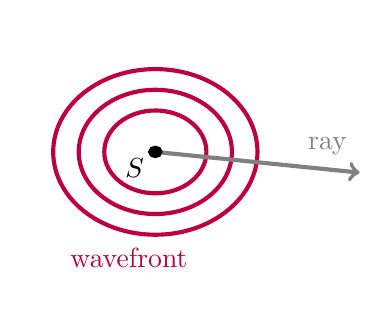
\begin{tikzpicture}
            \tikzstyle{every path}=[line width=1.5pt]
            \begin{axis}[
                ytick=\empty,
                xtick=\empty,
                samples=1000,
                axis line style={draw=none},
                enlargelimits=false,
                height=5cm,
                xmin=-1, xmax=12,
                ymin=-1, ymax=12
            ]
                \draw[draw=purple] (axis cs: 4, 6) circle [radius=2];
                \draw[draw=purple] (axis cs: 4, 6) circle [radius=3];
                \draw[draw=purple] (axis cs: 4, 6) circle [radius=4] node[midway, above= 0.5cm, right=0.4cm,purple] {wavefront};
                \draw[->,gray] (4,6) -- (12,5) node[midway, above=0.2cm, right=0.5cm] {ray};
                \draw[fill=black] (4,6) circle (0.2) node[below=0.2cm, left] {$S$};
            \end{axis}
        \end{tikzpicture}
    \end{minipage}
    \hfill
    \begin{minipage}[b] {0.6\textwidth}
        \begin{equation}
            v = \sqrt{\frac{B}{\rho}} = 343 \text{ m/s} \tag{speed of sound in air}\label{eq:soundSpeed}
        \end{equation}
        As sound waves pass through the air, areas of compression and and expansion form,
        in which we can find the speed by finding $B$, the rate of change of pressure over a volume,
        and $\rho$ the density of the medium.
    \end{minipage}

    \noindent \\ Since the speed of the wave is determined by its medium, not frequency,
    we can find the wavelength using the same formula from CH16 ($\lambda = \frac{v}{f} = \frac{343}{f}$).
    We can find the change in pressure caused by sound waves:
    \begin{equation}
       \Delta \rho = \Delta \rho_m \sin(kx - \omega t)
    \end{equation}
    Where the pressure amplitude is:
    \begin{equation}
     \Delta \rho_m = (v \rho \omega)s_m
    \end{equation}

    \noindent \\ Moving away from the source, the intensity of sound waves gradually decreases.
    \textbf{Intensity} (W/\text{m}$^{2}$) is the average power of a sound wave carries per unit area:

    \begin{equation}
        I = \frac{1}{2} \rho v \omega^2 s_{m}^2 \tag{intensity}\label{eq:intensity}
    \end{equation}

    \noindent We can find the intensity at any distance $r$ away from the source using the formula:
    \begin{equation}
        I = \frac{P_s}{4 \pi r^2} \tag{intensity at distance r}
    \end{equation}

    \noindent Note that intensity is proportional to the pressure squared
    ($I \propto \rho^2$).
    However, we measure \textbf{sound level} in decibels (dB) using a logarithmic scale
    where $I_0$ is the standard reference intensity ( $10^{-12}$ W/m^2).

    \begin{equation}
        \beta = (10 \text{dB}) \log \frac{I}{I_0} \tag{sound level}
    \end{equation}

    \noindent Sources of sound waves are not always stationary,
    in fact their velocity changes their perceived frequency.

     \hfill
    \begin{minipage}[b]{0.25\textwidth}
        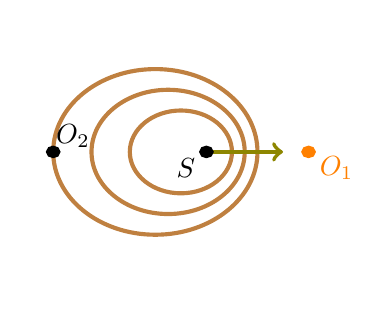
\begin{tikzpicture}
            \tikzstyle{every path}=[line width=1.5pt]
            \begin{axis}[
                ytick=\empty,
                xtick=\empty,
                samples=1000,
                axis line style={draw=none},
                enlargelimits=false,
                height=5cm,
                xmin=-1, xmax=12,
                ymin=-1, ymax=12
            ]
                \draw[draw=brown] (axis cs: 5, 6) circle [radius=2];
                \draw[draw=brown] (axis cs: 4.5, 6) circle [radius=3];
                \draw[draw=brown] (axis cs: 4, 6) circle [radius=4];
                \draw[->,olive] (6,6) -- (9,6);
                \draw[fill=black] (6,6) circle (0.2) node[below=0.2cm, left] {$S$};
                \draw[orange, fill=orange] (10,6) circle (0.2) node[orange, below=0.2cm, right] {$O_1$};
                \draw[black, fill=black] (0,6) circle (0.2) node[black, above=0.2cm, right=-3] {$O_2$};
            \end{axis}
        \end{tikzpicture}
    \end{minipage}
    \hfill
    \begin{minipage}[b] {0.7\textwidth}
        Where $v_o$ is the velocity of the observer, and $v_s$ is the velocity of the source.
        Frequency changes:
        \begin{equation}
            f' = f \frac{v \pm v_o}{v \mp v_s }  \tag{Doppler Effect}\label{doppler}
        \end{equation}

        The wavefronts show that the frequency increases as $\Delta x$ decreases, and vice versa.
    \end{minipage}

    \noindent \\
    With this in mind, the top equation is addition if $v_0$ is going towards the source,
    while the bottom is negative if $v_s$ is moving towards the observer.
    The signs switch if they go in the other direction.

   \newpage
    \noindent \textbf{Chapter 17 - Waves II}
    \noindent \\
\end{document}

